\documentclass[12pt,a4paper,openright]{mwrep}

\usepackage{lmodern}
\usepackage[T1]{polski}
\usepackage[utf8]{inputenc}

\usepackage[a4paper,
            tmargin=2cm,
            bmargin=2cm,
            lmargin=2cm,
            rmargin=2cm,
            bindingoffset=0cm]{geometry}

\usepackage{tocloft}
\usepackage{hyperref}

\usepackage{amsmath}
\usepackage{amssymb}
\usepackage{siunitx}

\usepackage{listings}

\usepackage{graphicx}
\usepackage{subfig}
\usepackage{float}
\usepackage{booktabs}

\hypersetup{
    colorlinks,
    citecolor=black,
    filecolor=black,
    linkcolor=black,
    urlcolor=black
}

\newtheorem{definition}{Def}

\begin{document}

\title{%
Technika cyfrowa\\
Sprawozdanie 1\\
}

\author{\\Jan Chyczyński\\Błażej Nowicki
\\Bartłomiej Słupik\\Przemysław Węglik}

\date{\today}

\maketitle

\chapter{Zadanie 1a}

\section{Wstęp}
Zadanie polega na zaprojektowaniu układu realizującego 
funkcję logiczną:
\begin{align*}
    Y = \overline{A}C + B(A + B)
\end{align*}
Układ można zrealizować wyłącznie dzięki użyciu bramek NAND
ponieważ bramka NAND jest systemem funkcjonalnie pełnym tzn.
korzystając wyłącznie z niej można przedstawić dowolną funkcję
boolowską.

\section{Rozwiązanie teoretyczne}
Pierwszym krokiem jest przekształcenie wyrażenie do zawierającego
wyłączenie operacje NAND.
\begin{align*}
    Y &= \overline{A}C + B(A + B) \\
    &= \overline{A}C + B \\
    &= \overline{\overline{\overline{A}C}\overline{B}}
\end{align*}

\section{Symulacja w programie Multisim}
Układ zbudowano w dwóch wersjach: pierwszej, z ręcznymi przełącznikami 
pozwalającymi na zmianę stanu A, B i C oraz drugiej, z generatorami sygnału
i oscyloskopem.

\begin{figure}[H]
    \centering
    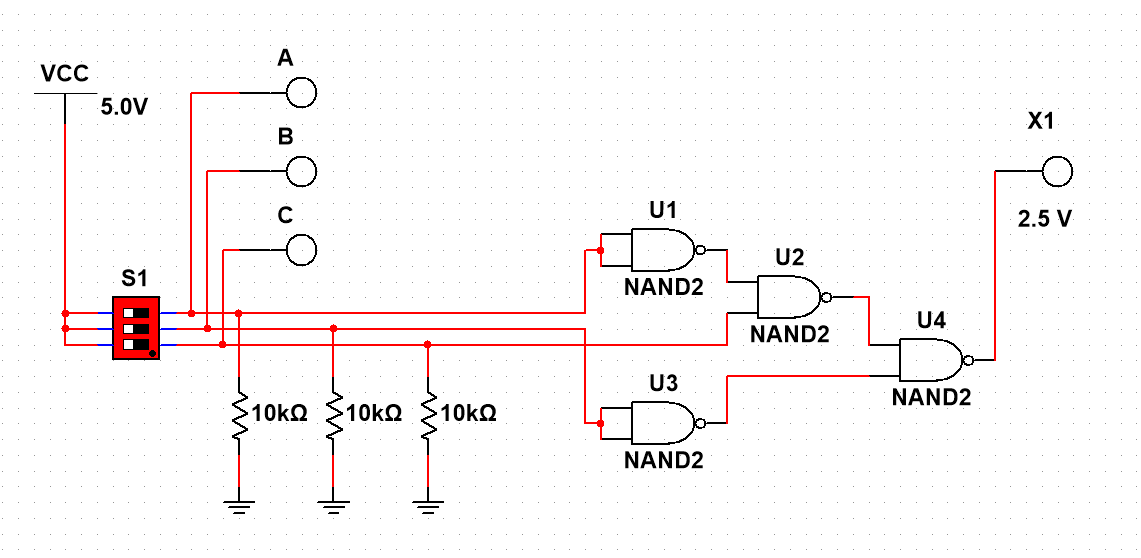
\includegraphics[width=1\textwidth]{images/1a_circuit_simple.png}
    \caption{Układ z ręcznymi przełącznikami}
    \label{rys:1a_circuit_simple}
\end{figure}

\begin{figure}[H]
    \centering
    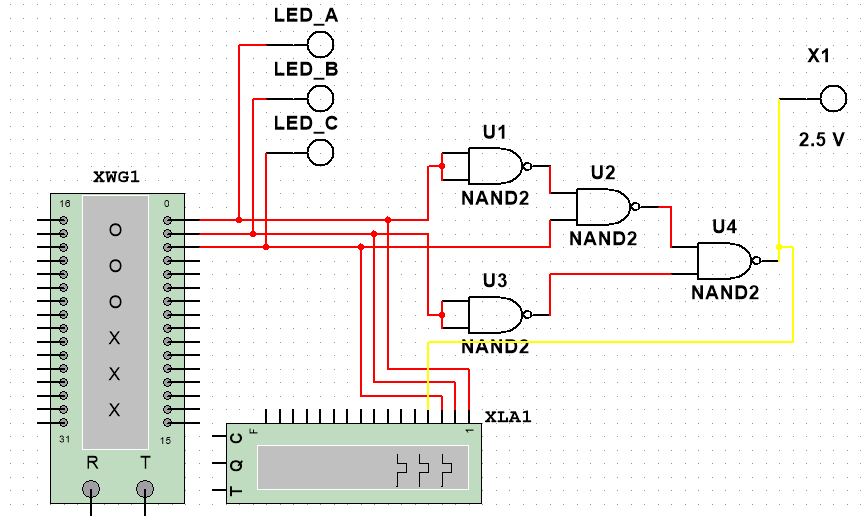
\includegraphics[width=1\textwidth]{images/1a_circuit_word_generator.png}
    \caption{Układ z generatorami i oscyloskopem}
    \label{rys:1a_circuit_with_generators}
\end{figure}

\begin{figure}[H]
    \centering
    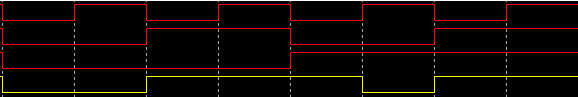
\includegraphics[width=0.8\textwidth]{images/1a_timeseries.png}
    \caption{Przebieg czasowy sygnałów. Od góry: A, B, C, Y}
    \label{rys:1a_timeseries}
\end{figure}

\newpage
\section{Wnioski}
\begin{enumerate}
    \item Dzięki prawom logiki możemy uprosić skomplikowane wyrażenia
    w taki sposób, aby używały mniejszej ilości operacji logicznych.
    \item Przedstawienie funkcji logicznej tylko za pomocą bramek NAND
    ma praktyczne zastosowanie, ponieważ komeryjnie dostępne chipy często
    zawierają kilka bramek tego samego rodzaju (np. 4xNAND, 4xOR itp.).
    Dzięki uproszczeniu układu do bramek NAND, możemy go skonstruować
    w rzeczywistościu używając tylko jednego chipu 4xNAND zamiast
    trzech różnych: 4xNOT, 4xOR i 4xAND.
    \item Podana funkcja logiczna po drobnym przekształceniu
    \begin{align*}
        Y = \overline{A}C + B(A + B) = \overline{A}C + B
    \end{align*}
    przedstawia równanie charakterystyczne przerzutnika 
    asynchronicznego typu RS. 
    Po podstawieniach
    \begin{align*}
        A &= R\\
        B &= S\\
        C &= Q_{n-1}\\
        Y &= Q_{n}\\
    \end{align*}
        
    otrzymujemy
    \begin{align*}
        Q_{n} = S + \overline{R}Q_{n-1}
    \end{align*}
\end{enumerate}



\end{document}
